

\section{Preparation}

\noindent
This chapter covers the following ideas. When you create your lesson plan, it should contain examples which illustrate these key ideas. Before you take the quiz on this unit, meet with another student out of class and teach each other from the examples on your lesson plan. 

\begin{enumerate}

\item Construct visualizations of matrices related to vector fields. Explain how eigenvalues and eigenvectors relate to vector fields.
\item Explain how to generalize the derivative to a matrix. Use this
  generalization to locate optimal values of a function using the second derivative test. Explain the role of eigenvalues and eigenvectors in the second derivative test.
\item Describe a Markov process. Explain what a steady-state solution is and how it relates to eigenvectors of the transition matrix.
\item Find the currents in an electrical system involving batteries and resistors, using both Gaussian elimination and Cramer's rule.
\item Find interpolating polynomials. Generalize this curve-fitting process to solve the least squares regression problem of fitting a line to a set of data.
\item Find bases for the column space, row space, and null space of a matrix and its transpose by row reducing $A$ and $A^T$. Use these bases to find the coordinates of vectors relative to the bases.

\end{enumerate}



%%% Local Variables: 
%%% mode: latex
%%% TeX-master: "../linear-algebra"
%%% End: 


Here are the preparation problems for this unit.  All of these problems come from this book (not Schaum's Outlines).  Remember that solutions appear at the end of each chapter.

%Day 1 we'll only look at matrix multiplication in class.  I'll introduce vector addition, scalar multiplication, the dot product, and then go to linear combinations. This leads immediately to matrix multiplication. Next we will focus on systems of equations and how to solve them.  I'll show how systems can be written in 4 ways, and then reduce a 2 by 2 system.  The next day we will focus on larger systems, and introduce rank and independence.  The next day I'll add in determinants and inverses, and hopefully get to eigenvalues and eigenvectors.   


\begin{center}
\begin{tabular}{ll|l}
\multicolumn{2}{c}{Preparation Problems (\href{http://ilearn.byui.edu/bbcswebdav/institution/Physical\_Sci\_Eng/Mathematics/Personal\%20Folders/WoodruffB/341/2-Applications-Preparation-Solutions.pdf}{click for solutions})}
&
Webcasts 
(
\href{http://ilearn.byui.edu/bbcswebdav/institution/Physical\_Sci\_Eng/Mathematics/Personal\%20Folders/WoodruffB/341/2-Applications-videos.pdf}{pdf copy}
)\\
\hline\hline
Day 1&
1b,
1g,
2c,
3b
&
\href{http://ilearn.byui.edu/bbcswebdav/institution/Physical\_Sci\_Eng/Mathematics/Personal\%20Folders/WoodruffB/341/2-Applications-video-01.wmv}{1},
\href{http://ilearn.byui.edu/bbcswebdav/institution/Physical\_Sci\_Eng/Mathematics/Personal\%20Folders/WoodruffB/341/2-Applications-video-02.wmv}{2},
\href{http://ilearn.byui.edu/bbcswebdav/institution/Physical\_Sci\_Eng/Mathematics/Personal\%20Folders/WoodruffB/341/2-Applications-video-03.wmv}{3}
\\ \hline
Day 2&
4b,
5b,
5d,
6b
&
\href{http://ilearn.byui.edu/bbcswebdav/institution/Physical\_Sci\_Eng/Mathematics/Personal\%20Folders/WoodruffB/341/2-Applications-video-04.wmv}{4},
\href{http://ilearn.byui.edu/bbcswebdav/institution/Physical\_Sci\_Eng/Mathematics/Personal\%20Folders/WoodruffB/341/2-Applications-video-05.wmv}{5},
\href{http://ilearn.byui.edu/bbcswebdav/institution/Physical\_Sci\_Eng/Mathematics/Personal\%20Folders/WoodruffB/341/2-Applications-video-06.wmv}{6}
\\ \hline
Day 3&
6e,
7a,
7b,
8b
&
\href{http://ilearn.byui.edu/bbcswebdav/institution/Physical\_Sci\_Eng/Mathematics/Personal\%20Folders/WoodruffB/341/2-Applications-video-07.wmv}{7},
\href{http://ilearn.byui.edu/bbcswebdav/institution/Physical\_Sci\_Eng/Mathematics/Personal\%20Folders/WoodruffB/341/2-Applications-video-08.wmv}{8},
\href{http://ilearn.byui.edu/bbcswebdav/institution/Physical\_Sci\_Eng/Mathematics/Personal\%20Folders/WoodruffB/341/2-Applications-video-09.wmv}{9}
\\ \hline
Day 4&
8c,
9b,
10b,
11b
&
\href{http://ilearn.byui.edu/bbcswebdav/institution/Physical\_Sci\_Eng/Mathematics/Personal\%20Folders/WoodruffB/341/2-Applications-video-10.wmv}{10},
\href{http://ilearn.byui.edu/bbcswebdav/institution/Physical\_Sci\_Eng/Mathematics/Personal\%20Folders/WoodruffB/341/2-Applications-video-11.wmv}{11}
\\ \hline
Day 6&
Lesson Plan,
Quiz, Start Project &
\\ \hline
\end{tabular}
\end{center}






The problems listed below are found in this book.
\begin{center}
\begin{tabular}{|l|l|l|l|l|}
\hline
Concept&Suggestions&Relevant Problems\\ \hline
Vector Fields&&\ref{vectorfields}\\ \hline
Kirchoff's Laws&&\ref{kirchoff}\\ \hline
Cramer's Rule&&\ref{cramer}\\ \hline
Interpolating Polynomials&&\ref{interpolating}\\ \hline
Least Square Regression&&\ref{regression}\\ \hline
2nd Derivative Test&&\ref{seconddertest}\\ \hline
Stochastic Processes&&\ref{stochastic}\\ \hline
Column and Row Spaces&&\ref{colandrowspace},\ref{coordinates}\\ \hline
Null Space and Projections&&\ref{nullspace},\ref{projections}\\ \hline
\end{tabular}
\end{center}












\section{Problems}
%The problems listed below are found in this book.
%\begin{center}
%\begin{tabular}{|l|l|l|l|l|}
%\hline
%Concept&Suggestions&Relevant Problems\\ \hline
%Kirchoff's Laws&&\ref{kirchoff}\\ \hline
%Cramer's Rule&&\ref{cramer}\\ \hline
%Interpolating Polynomials&&\ref{interpolating}\\ \hline
%Least Square Regression&&\ref{regression}\\ \hline
%Stochastic Processes&&\ref{stochastic}\\ \hline
%2nd Derivative Test&&\ref{seconddertest}\\ \hline
%\end{tabular}
%\end{center}


\begin{enumerate}

\item  {\bf Vector Fields:} \label{vectorfields}For each of the following vector fields, (1) construct a rough plot of the field by graphing the vectors at the 8 points surrounding the origin, (2) find the eigenvalues and eigenvectors, and if real (3) add to your plot the eigenvectors and some flow lines (curves representing the path of motion). Check your work using Sage.
\begin{enumerate}
\begin{multicols}{2}
	\item $F(x,y) = (2x+y,x+2y)$
	\item $F(x,y) = (2x+4y,4x+2y)$
	\item $F(x,y) = (-y,x)$
	\item $F(x,y) = (2x+3y,x+4y)$
	\item $F(x,y) = (2x+3y,4x+1y)$
	\item $F(x,y) = (y,-x)$
	\item $F(x,y) = (x+y,-x+y)$
	\item $F(x,y) = (x-y,x-y)$
	\item $F(x,y) = (x-y,2x-2y)$
	\item $F(x,y) = (-x-y,x-y)$
\end{multicols}
\end{enumerate}


\item  {\bf Kirchoff's Laws:} Consider the following electrical systems. Use the given values to find the current in each wire. \label{kirchoff}

\centerline{\renewcommand{\myscale}{.3}
\begin{tikzpicture}[scale=\myscale,inner sep=1pt]
%\draw[help lines,step=1cm] (0,0) grid (12,6);

%Source - like a battery
\node[label=right:$E$] at (0,3) 
{{\begin{tikzpicture}[scale=\myscale]
%	\useasboundingbox (-.5,-3) rectangle (.5,3);
	\draw (0,0) circle (1cm);
	\draw (.3,.5) -- (-.3,.5);
	\draw (0,.2) -- (0,.8);
	\draw (.3,-.5) -- (-.3,-.5);
	\draw (0,1) -- (0,3);
	\draw (0,-1) -- (0,-3);
	\end{tikzpicture}
}};

%Resistor
\node[label=right:$R_2$] at (6,3) 
{{\begin{tikzpicture}[scale=\myscale]
%	\useasboundingbox (0,-3) rectangle (0,3);
	\draw (0,-3) -- ++(0,1.8) -- ++(.5,.2) 
		-- ++(-1,.4) -- ++(1,.4)
		-- ++(-1,.4) -- ++(1,.4)
		-- ++(-1,.4) -- ++(.5,.2)
		-- ++(0,1.8) ;
	\end{tikzpicture}
}};

%Resistor
\node[label=above:$R_1$] at (3,0) 
{{\begin{tikzpicture}[scale=\myscale,rotate=90]
%	\useasboundingbox (0,-3) rectangle (0,3);
	\draw (0,-3) -- ++(0,1.8) -- ++(.5,.2) 
		-- ++(-1,.4) -- ++(1,.4)
		-- ++(-1,.4) -- ++(1,.4)
		-- ++(-1,.4) -- ++(.5,.2)
		-- ++(0,1.8) ;
	\end{tikzpicture}
}};

%Resistor
\node[label=right:$R_3$] at (12,3) 
{{\begin{tikzpicture}[scale=\myscale,rotate=0]
%	\useasboundingbox (0,-3) rectangle (0,3);
	\draw (0,-3) -- ++(0,1.8) -- ++(.5,.2) 
		-- ++(-1,.4) -- ++(1,.4)
		-- ++(-1,.4) -- ++(1,.4)
		-- ++(-1,.4) -- ++(.5,.2)
		-- ++(0,1.8) ;
	\end{tikzpicture}
}};

%Straight Path
\node at (3,6) 
{{\begin{tikzpicture}[scale=\myscale,rotate=90]
	\draw (0,-3) -- (0,3);
	\end{tikzpicture}
}};

%Straight Path
\node at (9,6) 
{{\begin{tikzpicture}[scale=\myscale,rotate=90]
	\draw (0,-3) -- (0,3);
	\end{tikzpicture}
}};

%Straight Path
\node at (9,0) 
{{\begin{tikzpicture}[scale=\myscale,rotate=90]
	\draw (0,-3) -- (0,3);
	\end{tikzpicture}
}};


%Arrow to represent Current
\node[label=above:$i_1$] at (3,6) 
{{\begin{tikzpicture}[scale=\myscale,rotate=-90]
%	\useasboundingbox (0,-.4) rectangle (0,.4);
	\filldraw (0,.4) -- (-.2,-.4) -- (0,-.3) -- (.2,-.4);
	\end{tikzpicture}
}};

%Arrow to represent Current
\node[label=right:$i_2$] at (6,5) 
{{\begin{tikzpicture}[scale=\myscale,rotate=180]
%	\useasboundingbox (0,-.4) rectangle (0,.4);
	\filldraw (0,.4) -- (-.2,-.4) -- (0,-.3) -- (.2,-.4);
	\end{tikzpicture}
}};

%Arrow to represent Current
\node[label=above:$i_3$] at (9,6) 
{{\begin{tikzpicture}[scale=\myscale,rotate=-90]
%	\useasboundingbox (0,-.4) rectangle (0,.4);
	\filldraw (0,.4) -- (-.2,-.4) -- (0,-.3) -- (.2,-.4);
	\end{tikzpicture}
}};

%Node
\node at (6,6) 
{{\begin{tikzpicture}[scale=\myscale,rotate=-90]
%	\useasboundingbox (0,-.4) rectangle (0,.4);
	\filldraw (0,0) circle (.15cm);
	\end{tikzpicture}
}};

%Node
\node at (6,0) 
{{\begin{tikzpicture}[scale=\myscale,rotate=-90]
%	\useasboundingbox (0,-.4) rectangle (0,.4);
	\filldraw (0,0) circle (.15cm);
	\end{tikzpicture}
}};

\end{tikzpicture}

\renewcommand{\myscale}{.3}
\begin{tikzpicture}[scale=\myscale,inner sep=1pt]
%\draw[help lines,step=1cm] (0,0) grid (18,6);

%Source - like a battery
\node[label=right:$E$] at (0,3) 
{{\begin{tikzpicture}[scale=\myscale]
%	\useasboundingbox (-.5,-3) rectangle (.5,3);
	\draw (0,0) circle (1cm);
	\draw (.3,.5) -- (-.3,.5);
	\draw (0,.2) -- (0,.8);
	\draw (.3,-.5) -- (-.3,-.5);
	\draw (0,1) -- (0,3);
	\draw (0,-1) -- (0,-3);
	\end{tikzpicture}
}};

%Resistor
\node[label=right:$R_2$] at (6,3) 
{{\begin{tikzpicture}[scale=\myscale]
%	\useasboundingbox (0,-3) rectangle (0,3);
	\draw (0,-3) -- ++(0,1.8) -- ++(.5,.2) 
		-- ++(-1,.4) -- ++(1,.4)
		-- ++(-1,.4) -- ++(1,.4)
		-- ++(-1,.4) -- ++(.5,.2)
		-- ++(0,1.8) ;
	\end{tikzpicture}
}};

%Resistor
\node[label=above:$R_1$] at (3,0) 
{{\begin{tikzpicture}[scale=\myscale,rotate=90]
%	\useasboundingbox (0,-3) rectangle (0,3);
	\draw (0,-3) -- ++(0,1.8) -- ++(.5,.2) 
		-- ++(-1,.4) -- ++(1,.4)
		-- ++(-1,.4) -- ++(1,.4)
		-- ++(-1,.4) -- ++(.5,.2)
		-- ++(0,1.8) ;
	\end{tikzpicture}
}};

%Resistor
\node[label=above:$R_3$] at (9,6) 
{{\begin{tikzpicture}[scale=\myscale,rotate=90]
%	\useasboundingbox (0,-3) rectangle (0,3);
	\draw (0,-3) -- ++(0,1.8) -- ++(.5,.2) 
		-- ++(-1,.4) -- ++(1,.4)
		-- ++(-1,.4) -- ++(1,.4)
		-- ++(-1,.4) -- ++(.5,.2)
		-- ++(0,1.8) ;
	\end{tikzpicture}
}};

%Resistor
\node[label=right:$R_4$] at (12,3) 
{{\begin{tikzpicture}[scale=\myscale,rotate=0]
%	\useasboundingbox (0,-3) rectangle (0,3);
	\draw (0,-3) -- ++(0,1.8) -- ++(.5,.2) 
		-- ++(-1,.4) -- ++(1,.4)
		-- ++(-1,.4) -- ++(1,.4)
		-- ++(-1,.4) -- ++(.5,.2)
		-- ++(0,1.8) ;
	\end{tikzpicture}
}};

%Resistor
\node[label=right:$R_5$] at (18,3) 
{{\begin{tikzpicture}[scale=\myscale,rotate=0]
%	\useasboundingbox (0,-3) rectangle (0,3);
	\draw (0,-3) -- ++(0,1.8) -- ++(.5,.2) 
		-- ++(-1,.4) -- ++(1,.4)
		-- ++(-1,.4) -- ++(1,.4)
		-- ++(-1,.4) -- ++(.5,.2)
		-- ++(0,1.8) ;
	\end{tikzpicture}
}};

%Resistor
\node[label=above:$R_6$] at (9,0) 
{{\begin{tikzpicture}[scale=\myscale,rotate=90]
%	\useasboundingbox (0,-3) rectangle (0,3);
	\draw (0,-3) -- ++(0,1.8) -- ++(.5,.2) 
		-- ++(-1,.4) -- ++(1,.4)
		-- ++(-1,.4) -- ++(1,.4)
		-- ++(-1,.4) -- ++(.5,.2)
		-- ++(0,1.8) ;
	\end{tikzpicture}
}};









%Straight Path
\node at (3,6) 
{{\begin{tikzpicture}[scale=\myscale,rotate=90]
	\draw (0,-3) -- (0,3);
	\end{tikzpicture}
}};

%Straight Path
\node at (15,6) 
{{\begin{tikzpicture}[scale=\myscale,rotate=90]
	\draw (0,-3) -- (0,3);
	\end{tikzpicture}
}};

%Straight Path
\node at (15,0) 
{{\begin{tikzpicture}[scale=\myscale,rotate=90]
	\draw (0,-3) -- (0,3);
	\end{tikzpicture}
}};






%Arrow to represent Current
\node[label=above:$i_1$] at (3,6) 
{{\begin{tikzpicture}[scale=\myscale,rotate=-90]
%	\useasboundingbox (0,-.4) rectangle (0,.4);
	\filldraw (0,.4) -- (-.2,-.4) -- (0,-.3) -- (.2,-.4);
	\end{tikzpicture}
}};

%Arrow to represent Current
\node[label=right:$i_2$] at (6,5) 
{{\begin{tikzpicture}[scale=\myscale,rotate=180]
%	\useasboundingbox (0,-.4) rectangle (0,.4);
	\filldraw (0,.4) -- (-.2,-.4) -- (0,-.3) -- (.2,-.4);
	\end{tikzpicture}
}};

%Arrow to represent Current
\node[label=above:$i_3$] at (7,6) 
{{\begin{tikzpicture}[scale=\myscale,rotate=-90]
%	\useasboundingbox (0,-.4) rectangle (0,.4);
	\filldraw (0,.4) -- (-.2,-.4) -- (0,-.3) -- (.2,-.4);
	\end{tikzpicture}
}};

%Arrow to represent Current
\node[label=right:$i_4$] at (12,5) 
{{\begin{tikzpicture}[scale=\myscale,rotate=180]
%	\useasboundingbox (0,-.4) rectangle (0,.4);
	\filldraw (0,.4) -- (-.2,-.4) -- (0,-.3) -- (.2,-.4);
	\end{tikzpicture}
}};

%Arrow to represent Current
\node[label=above:$i_5$] at (15,6) 
{{\begin{tikzpicture}[scale=\myscale,rotate=-90]
%	\useasboundingbox (0,-.4) rectangle (0,.4);
	\filldraw (0,.4) -- (-.2,-.4) -- (0,-.3) -- (.2,-.4);
	\end{tikzpicture}
}};

%Arrow to represent Current
\node[label=above:$i_6$] at (11,0) 
{{\begin{tikzpicture}[scale=\myscale,rotate=90]
%	\useasboundingbox (0,-.4) rectangle (0,.4);
	\filldraw (0,.4) -- (-.2,-.4) -- (0,-.3) -- (.2,-.4);
	\end{tikzpicture}
}};








%Node
\node at (6,6) 
{{\begin{tikzpicture}[scale=\myscale,rotate=-90]
%	\useasboundingbox (0,-.4) rectangle (0,.4);
	\filldraw (0,0) circle (.15cm);
	\end{tikzpicture}
}};

%Node
\node at (6,0) 
{{\begin{tikzpicture}[scale=\myscale,rotate=-90]
%	\useasboundingbox (0,-.4) rectangle (0,.4);
	\filldraw (0,0) circle (.15cm);
	\end{tikzpicture}
}};

%Node
\node at (12,0) 
{{\begin{tikzpicture}[scale=\myscale,rotate=-90]
%	\useasboundingbox (0,-.4) rectangle (0,.4);
	\filldraw (0,0) circle (.15cm);
	\end{tikzpicture}
}};

%Node
\node at (12,6) 
{{\begin{tikzpicture}[scale=\myscale,rotate=-90]
%	\useasboundingbox (0,-.4) rectangle (0,.4);
	\filldraw (0,0) circle (.15cm);
	\end{tikzpicture}
}};

\end{tikzpicture}
}
\begin{multicols}{2}
\begin{enumerate}

\item $E=12, R_1=2,R_2=2, R_3=2$.
\item $E=12, R_1=2,R_2=3, R_3=3$.
\item $E=12, R_1=2,R_2=3, R_3=6$.
\item $E=12, R_1=1,R_2=2, R_3=2$.
\item $E=9, R_1=3,R_2=1, R_3=2$.
\item $E=6, R_1=1,R_2=1, R_3=2$.
\end{enumerate}
\end{multicols}


\begin{enumerate} \setcounter{enumii}{6}
\item $E=12$, $R_1=1$, $R_2=1$, $R_3=1$, $R_4=1$, $R_5=1$, $R_6=1$
\item $E=12$, $R_1=2$, $R_2=1$, $R_3=3$, $R_4=4$, $R_5=2$, $R_6=3$
\end{enumerate}


\item  {\bf Cramer's Rule:}\label{cramer}Use Cramer's rule to find solutions to the following linear systems. If Cramer's rule fails, explain why.

\begin{enumerate}
\begin{multicols}{2}
\item $2x+3y=0, x-2y=1$
\item $x+y=2, x-y=3$
\item $3x+y=6, x+3y=2$
\item $2x+y=1, 4x+2y=2$
\item $x+y=0, 2x-y+z=1, x+z=0$
\item $x+2y=3, x-y+z=0, x+3y+z=1$
\item $y+2z=1, x-z=3, 2x+y=1$
\end{multicols}
\item Re solve any of the problems from problems \ref{kirchoff} or \ref{interpolating} using Cramer's rule.
\end{enumerate}





\item {\bf Interpolating Polynomials:} \label{interpolating}In each of the following scenarios, find a polynomial of least degree which passes through the given points. Verify your result graphically by plotting the points and the polynomial.
\begin{enumerate}
\begin{multicols}{3}
\item $(1,2),(3,3)$ 			
\item $(0,1),(2,3),(-1,4)$  
\item $(1,1),(2,2),(-1,5)$   
\item $(1,2),(3,3),(5,6)$ 			
\item $(1,2),(3,3),(5,5)$ 
\item $(0,1),(1,3),(-1,4),(2,4)$ 
\end{multicols}
\item Select any number of points (with varying $x$ values), and find the interpolating polynomial which goes through them. Check your answer by plugging the points into your polynomial.
\item Open up a spread sheet program (like Microsoft Excel). Make a column of $x$ values and a column of $y$ values. Create a scatter plot of the data and then on your scatter plot add the interpolating polynomial as well as its equation. You can use this to check your answer on any problem you create yourself.
\end{enumerate}



\item {\bf Regression:} \label{regression}For each set of data points, find an equation of the least squares regression line. Plot the points and the line on the same axes. Does the line appear to be the best fit?

\begin{enumerate}
\begin{multicols}{3}
\item $(0,0),(1,3),(1,2)$
\item $(1,1),(2,1),(3,2)$
\item $(1,2),(3,0),(5,1)$
\item $(0,0),(1,3),(1,2),(4,5)$
\item $(0,0),(1,3),(1,2),(4,-5)$
\item $(-1,2),(1,3),(2,5),(3,3)$
\end{multicols}
\item Challenge: Find an equation of the least squares regression parabola $y=a_0+a_1x+a_2x^2$ which passes through the points $(0,0),(1,3),(1,2),(4,5)$. [Hint, you will need a 4 by 3 matrix for $A$ instead of an $n$ by $2$. Use the transpose.]
\end{enumerate}




%\item Compute each integral by finding a partial fraction decomposition. 
%\begin{enumerate}
%\begin{multicols}{2}
%\item $\ds\int\frac{1}{(x-3)(x+2)}dx $%, \frac{A}{x-3}+\frac{B}{x+2}$         
%\item $\ds\int\frac{2x+3}{(x-3)(x+2)}dx$%, \frac{A}{x-3}+\frac{B}{x+2}$ 
%\item $\ds\int\frac{x}{(x+1)(x-2)}dx$%,  \frac{A}{x+1}+\frac{B}{x-2}$  
%\item $\ds\int\frac{x^2+2}{x^2(x-2)}dx$%, \frac{A}{x}+\frac{B}{x^2}+\frac{C}{x-2}$ 
%\item $\ds\int\frac{1}{(x^2+1)(x-2)}dx$%, \frac{Ax+B}{x^2+1}+\frac{C}{x-2}$
%\item $\ds\int\frac{x+1}{(x^2+1)x^2}dx$%, \frac{Ax+B}{x^2+1}+\frac{C}{x}+\frac{D}{x^2}$  
%\end{multicols}
%\end{enumerate}









\item {\bf Second Derivative Test:} \label{seconddertest}For each function, find the location of all critical points. Then use the second derivative test to determine if each critical point corresponds to a maximum, minimum, or saddle point. Graph the function in 3D to verify your results, and locate the eigenvectors and eigenvalues in the picture.
\begin{enumerate}
\begin{multicols}{2}
\item $f(x,y) = x^2+xy+y^2$
\item $f(x,y) = x^2+4xy+y^2$
\item $f(x,y) = x^2+2xy+y^2$
\item $f(x,y) = x^2-4x+y^2+2y+1$
\item $f(x,y) = x^2-2x+xy+y^2$
\item $f(x,y) = x^2+xy+3y^2$
\item $f(x,y) = x^3-3x+y^2-2y$ (2 critical points)
\item $f(x,y) = x^3-3x+y^3-3y^2$ (4 critical points)
\end{multicols}
\item $f(x,y,z)=x^2+xy+y^2+z^2-4z$ (the Hessian will be a 3 by 3 matrix)
\item Create your own function of the form $f(x,y)=Ax^2+Bxy+Cy^2+Dx+Ey+F$.  Find the critical points and determine if they correspond to a maximum, minimum, or saddle point. 
\item For what values of $A,B,C,D,E,F$ will $f(x,y)=Ax^2+Bxy+Cy^2+Dx+Ey+F$ have a critical point that corresponds to a minimum? a maximum? a saddle point? When will the second derivative test fail? How does $B^2-4AC$ relate to this problem? [Hint: the quadratic formula will prove useful in trying to find the eigenvalues symbolically.  How does the product of the eigenvalues relate to the determinant of the Hessian?]
\end{enumerate}







\item  {\bf Markov Processes:}\label{stochastic} In each scenario, write the transition matrix. If an initial state is given, then find the next two states. Finish by finding a steady state solution and use it to answer the question at the end.
%\begin{multicols}{2}
\begin{enumerate}

\item In a certain town, there are 3 types of land zones: residential, commercial, and industrial. The city has been undergoing growth recently, and the city has noticed the following trends.  Every 5 years, 10\% of the older residential land gets rezoned as commercial land, while 5\% gets rezoned as industrial.  The other 85\% remains residential.  For commercial land, 70\% remains commercial, while 10\% becomes residential and 20\% becomes industrial. For industrial land, 60\% remains industrial, while 25\% becomes commercial and 15\% becomes residential. Currently the percent of land in each zone is 40\% residential, 30\% commercial, and 30\% industrial. What will the percent distribution be in 5 years? In 10 years?  If this trend continues indefinitely, what percent of the land will eventually be residential?. 
\item Suppose we own a car rental company which rents cars in Idaho Falls and Rexburg. The last few weeks have shown a weekly trend that 60\% of the cars rented in Rexburg will remain in Rexburg (the other 40\% end up in IF), whereas 80\% of the cars rented in Idaho Falls will remain in Idaho Falls. If there are currently 60 cars in Rexburg and 140 cars in IF, how many will be in each city next week?  In two weeks? In three weeks? If this trend continues indefinitely, about how many cars should you expect to find in Rexburg each week?
\item Repeat the previous problem if 40\% of the cars rented in Rexburg will remain in Rexburg (the other 60\% end up in IF), whereas 80\% of the cars rented in Idaho Falls will remain in Idaho Falls.
\item Repeat the previous problem if 70\% of the cars rented in Rexburg will remain in Rexburg (the other 30\% end up in IF), whereas 80\% of the cars rented in Idaho Falls will remain in Idaho Falls.
\item A school cafeteria regularly offers 3 types of meals to its students. One of the meals is always a pizza/salad combo, One is always hamburgers and fries, and one is a daily special which changes daily. In an attempt to understand student preferences, the school discovered the following information. If a student has a hamburger one day, then there is a 30\% chance they will try the daily special the next day, and a 40\% percent chance they will have the salad bar.  If they have the salad bar, then there is a 30\% chance they'll switch to the daily special, and a 40\% chance they'll switch to the hamburger.  If the have the daily special, then there is a 50\% chance they'll get the daily special the next day, a 20\% chance they'll switch to pizza, and a 30\% chance they'll switch to hamburger.  If this trend continues, what percent of the students will eat each type of meal? 

[While this problem is highly rigged, there is a branch of applied mathematics which is studied by financial analysts call stochastic processes which models such a scenario. This modeling process can help predict how a new restaurant will perform in a city, sometimes predict stock market fluctuations, and more. The study of stochastic processes begins with a Markov chain and then introduces statistics and probability to help predict what happens when trends change.]
\end{enumerate}
%\end{multicols}




\item  {\bf Column and Row Spaces:} \label{colandrowspace}For each matrix, find the reduced row echelon form of both $A$ and $A^T$.  Use your results to give two bases for the column space. Then give two bases for the row space. If you feel like you have mastered row reduction, then please use a computer (practice using Sage) to do the row reduction for you so that you can focus on just being able to pick out the two different bases. 

\begin{enumerate}
\begin{multicols}{3}
\item 
$\begin{bmatrix}
 2 & 3 & 1 \\
 -3 & -5 & 3
\end{bmatrix}
$

\item
$
\begin{bmatrix}
 2 & 4 & 1 \\
 1 & 2 & 3
\end{bmatrix}
$

\item
$
\begin{bmatrix}
 1 & 2 & 3 \\
 2 & 0 & 1 \\
 -3 & -2 & -4
\end{bmatrix}
$

\item
$
\begin{bmatrix}
 1 & 3 & 2 \\
 2 & 1 & 0 \\
 -3 & -4 & -2
\end{bmatrix}
$

\item
$
\begin{bmatrix}
 2 & 1 & -2 & 4 \\
 1 & 3 & 0 & 5 \\
 -2 & 1 & 1 & 2
\end{bmatrix}
$

\item
$
\begin{bmatrix}
 0 & 1 & 2 & 3 \\
 2 & -1 & -4 & 0 \\
 -1 & 2 & 5 & 5
\end{bmatrix}
$

\end{multicols}
\end{enumerate}


\item  {\bf Coordinates of a vector relative to a basis:} \label{coordinates} For this problem, use the same matrices as problem 8.  From the columns of $A$, select a basis for the column space of $A$. Then give the coordinates of $\vec v$ and $\vec w$ relative to this basis, or explain why the vector is not in the column space of $A$.  
\begin{enumerate}
\begin{multicols}{3}
\item 
$\vec v = (2, 1)$ ,\\
$\vec w = (-1, 3)$


\item 
$\vec v = (6, 3)$ ,\\
$\vec w = (-1, 3)$

\item 
$\vec v = (3, -4, 1)$ ,\\
$\vec w = (-1, 3, 2)$

\item 
$\vec v = (3, -4, 1)$ ,\\
$\vec w = (3, -3, 0)$

\item 
$\vec v = (0, 8, 10)$ ,\\
$\vec w = (-13, -9, 2)$

\item 
$\vec v = (-7, 0, -12)$ ,\\
$\vec w = (-8, 11, -18)$
\end{multicols}
\end{enumerate}



\item  {\bf Null Space, Eigenspace, and Orthogonal Complement:} \label{nullspace}By finding the solutions to either $A\vec x=\vec 0$ (the null space), $(A-\lambda I)\vec x = \vec 0$ (an eigenspace), or $A^T\vec x = \vec 0$ (an orthogonal complement), find a basis and the dimension of the vector subspace requested.

$$
A= \begin{bmatrix}
 0 & -4 & -4 \\
 9 & 2 & -1 \\
 -3 & 0 & 1
\end{bmatrix}
,
B=\begin{bmatrix}
 2 & 4 & -4 & -7 \\
 3 & 6 & 1 & 0 \\
 -1 & -2 & 1 & 2 \\
 0 & 0 & 8 & 12
\end{bmatrix}
,
C=
\begin{bmatrix}
 2 & 0 & 4 & 2 \\
 -1 & -6 & 1 & -4 \\
 2 & -2 & 5 & 1
\end{bmatrix}
, 
D=
\begin{bmatrix}
 0 & 4 & 4 \\
 3 & -2 & -5 \\
 1 & 4 & 3 \\
 -2 & 0 & 2
\end{bmatrix}
$$

\begin{enumerate}
\begin{multicols}{2}
\item Find a basis for the null space of $A$.
\item Find a basis for the null space of $B$.
\item Find a basis for the null space of $C$.
\item Find a basis for the null space of $D$.
\end{multicols}
\item Find a basis for the set of vectors that are orthogonal to the columns of $A$.
\item Find a basis for the set of vectors that are orthogonal to the columns of $B$.
\item Find a basis for the set of vectors that are orthogonal to the columns of $C$.
\item Find a basis for the set of vectors that are orthogonal to the columns of $D$.

\item For
$
\begin{bmatrix}
 2 & -1 & 1 \\
 -1 & 2 & 1 \\
 -2 & -2 & 5
\end{bmatrix}
$, find a basis for the eigenspace corresponding to $\lambda = 3$.

\item For
$
\begin{bmatrix}
 -4 & 8 & 6 \\
 -9 & 14 & 9 \\
 6 & -8 & -4
\end{bmatrix}
$, find a basis for the eigenspace corresponding to $\lambda = 2$.




\end{enumerate}



\item {\bf Projections:} \label{projections}Let $\vec w$ be the projection of $\vec b$ onto the column space of $A$.  Find the coordinates of $\vec w$ relative to the columns of $A$. Then state the vector $\vec w$. Check that you are correct by showing that $\vec r = \vec b-\vec w$ is orthogonal to the columns of $A$ (i.e. show $A^T\vec r=\vec 0$). Compare to problem \ref{regression}
\begin{enumerate}
\item 
\begin{multicols}{3}

$A=
\begin{bmatrix}
\cl{1\\1\\1}&
\cl{0\\1\\1}
\end{bmatrix}
$, 
$\vec b = 
\begin{bmatrix}
\cl{0\\3\\2}
\end{bmatrix}
$

\item 
$A=
\begin{bmatrix}
\cl{1\\1\\1}&
\cl{1\\2\\3}
\end{bmatrix}
$, 
$\vec b = 
\begin{bmatrix}
\cl{1\\1\\2}
\end{bmatrix}
$


\item 
$A=
\begin{bmatrix}
\cl{1\\1\\1}&
\cl{1\\3\\5}
\end{bmatrix}
$, 
$\vec b = 
\begin{bmatrix}
\cl{2\\0\\1}
\end{bmatrix}
$


\item 
$A=
\begin{bmatrix}
\cl{1\\1\\1\\1}&
\cl{0\\1\\1\\4}
\end{bmatrix}
$, 
$\vec b = 
\begin{bmatrix}
\cl{0\\3\\2\\5}
\end{bmatrix}
$


\item 
$A=
\begin{bmatrix}
\cl{1\\1\\1\\1}&
\cl{0\\1\\1\\4}
\end{bmatrix}
$, 
$\vec b = 
\begin{bmatrix}
\cl{0\\3\\2\\-5}
\end{bmatrix}
$


\item 
$A=
\begin{bmatrix}
\cl{1\\1\\1\\1}&
\cl{-1\\1\\2\\3}
\end{bmatrix}
$, 
$\vec b = 
\begin{bmatrix}
\cl{2\\3\\5\\3}
\end{bmatrix}
$

\end{multicols}


\end{enumerate}


\end{enumerate}




\section{Projects}
\begin{enumerate}

%This will be updated shortly.  It will involve using the computer to explore how Sage finds basis vectors for a vector space. We'll explore the difference between using $A$ and $A^T$, and why a computer uses $A^T$ instead of $A$.  We'll give a reason for why one is called the standard or cannonical basis.
%
%Goal of project.  Learn how to determine if two basis for a vector space are the same.  Different computers give different basis.  The answers in the back of the book may be different.  A vector space is a huge collection of vectors, and there are infinitely many ways to give a basis for the vector space.  So how do we determine if two vector spaces are the same?  The idea is to use rref.  Once you have a basis, place the vectors in rows and row reduced the matrix.  When you are finished, you will have obtained a basis for the row space.  Any other vectors in this space must depend on these vectors, so if you place additional vectors in the matrix as additional rows, then again you should not obtain anything different.  If you start with a different basis, row reduce that matrix.  If it's rref is the same as the first, you have the same space.  If the rref's are not the same, you have a different space.
%
%Now I need to write this up so that they give me what I just said.



	\item Consider the matrices
$A=
\begin{bmatrix}
 2 & 4 & -4 & -7 \\
 3 & 6 & 1 & 0 \\
 -1 & -2 & 1 & 2 \\
 0 & 0 & 8 & 12
\end{bmatrix}
$ and 
$B=
\begin{bmatrix}
 -4 & -7 & 2 & 4 \\
 1 & 0& 3 & 6  \\
 1 & 2& -1 & -2  \\
 8 & 12& 0 & 0 
\end{bmatrix}
$. Because both matrices have the same columns (just in a different order), the column space of $A$ and the column space of $B$ both represent the same vector subspace. There are infinitely many vectors in this subspace, so there are infinitely many ways to find a basis. Is there a standard basis, one that we can compare any other basis to in an easy manner?  The problems below will help you discover this basis.

\begin{enumerate}
	\item \label{project2A} Find a basis for the column space of $A$ by selecting the pivot columns.
	\item \label{project2B} Find a basis for the column space of $B$ by selecting the pivot columns.
	\item Find a basis for the column space of $A$ by reducing $A^T$. 
	\end{enumerate}
	
	You should now have 3 different bases. The next 5 problems should all result in the same basis.
	\begin{enumerate}[resume]
	\item Find a basis for the column space of $B$ by reducing $B^T$.
	\item Let $C$ be a matrix whose columns are the basis vectors obtained in part (a). Row reduce the transpose to obtain a different basis. 
	\item Let $D$ be a matrix whose columns are the basis vectors obtained in part(b). Row reduce the transpose to obtain a different basis.
	\item Interchange the columns of $A$ in some other way.  Row reduce the transpose of your matrix to obtain a basis for the column space of $A$.
	\item Joe claims that a basis for the column space is 
	$\{(-5,3,1,12),(0,7,-1,8)\}$.  Is he correct?  To answer this, place his vectors in the columns of a matrix and then row reduce the transpose.  

      \item This basis is the basis Sage gives you when you ask for the column
space of a matrix.  Using Sage, compute the column space of $A$ and
$B$ using the \verb|column_space()| method (i.e., \verb|A.column_space()|).

\end{enumerate}

The basis obtained above is called the standard basis for the column
space of $A$. Because the rref of a matrix is unique, the standard
basis for a vector space will always be the same, no matter how the
vector space is described.  Any time someone gives you a basis for a vector subspace of $\mathbb{R}^n$, you can obtain the standard basis using the ideas above.  Just place the  vectors into the columns of matrix, and then reduce the transpose. Alternatively, just place the vectors into the rows of a matrix, and then reduce the matrix. 



 



\end{enumerate}


{
\section{Solutions}
\small
Here are the solutions

\begin{multicols}{2}
\begin{enumerate}
\item Vector Fields:  
\newcommand{\myvfwidth}{1.5in}
\begin{enumerate}
\item $3, (1,1),  5, (-1,1)$\\ 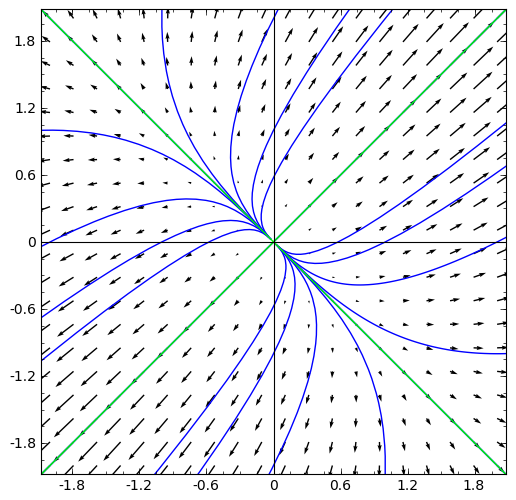
\includegraphics[width=\myvfwidth]{Applications/support/vfa}
\item $6, (1,1),  -2, (-1,1)$\\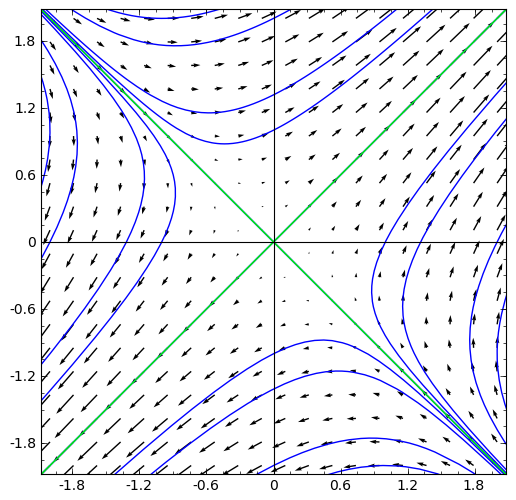
\includegraphics[width=\myvfwidth]{Applications/support/vfb}
\item $i, (i,1),  -i, (-i,1)$\\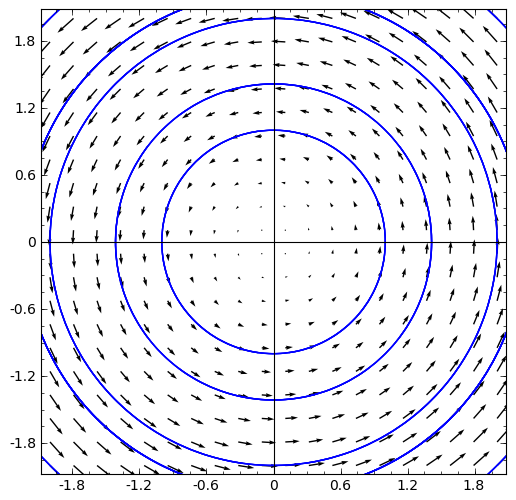
\includegraphics[width=\myvfwidth]{Applications/support/vfc}
\item $5, (1,1),  1, (-3,1)$\\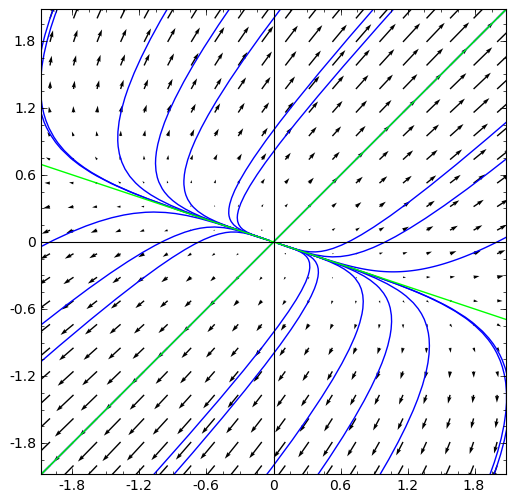
\includegraphics[width=\myvfwidth]{Applications/support/vfd}
\item $5, (1,1),  -2, (-3/4,1)$\\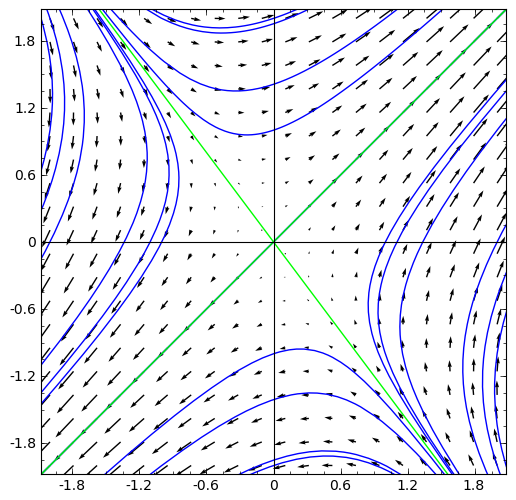
\includegraphics[width=\myvfwidth]{Applications/support/vfe}
\item $i, (-i,1),  -i, (i,1)$\\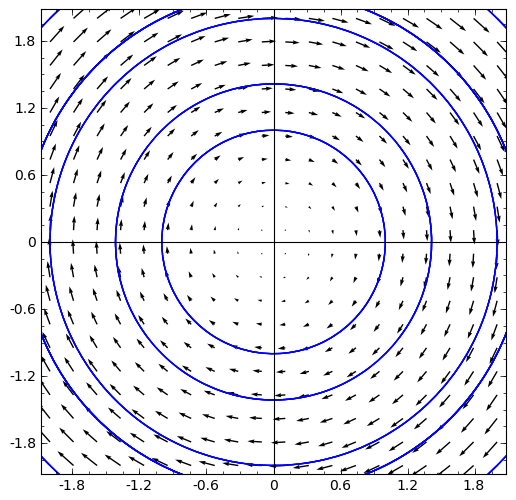
\includegraphics[width=\myvfwidth]{Applications/support/vff}
\item $1+i, (-i,1), 1-i, (i,1)$\\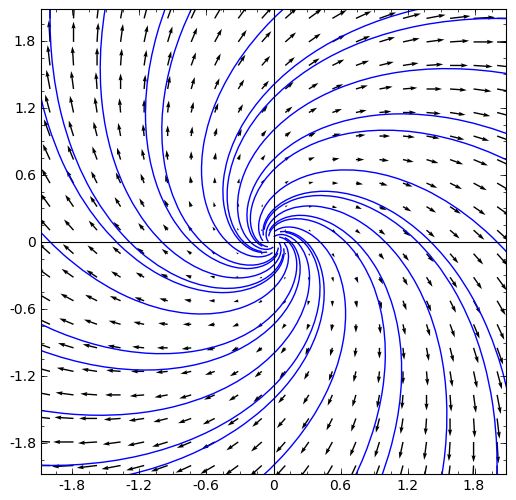
\includegraphics[width=\myvfwidth]{Applications/support/vfg}
\item $0, (1,1)$, there only one independent eigenvectors. \\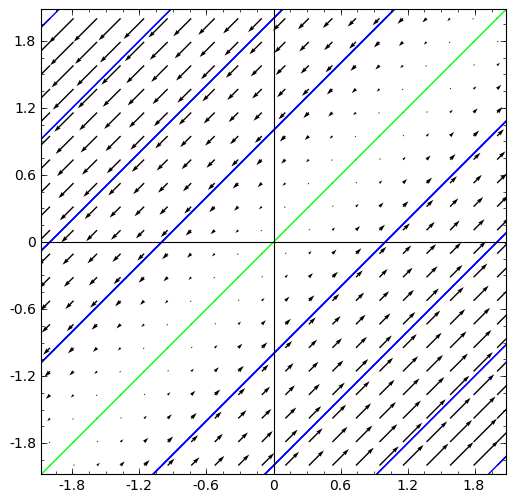
\includegraphics[width=\myvfwidth]{Applications/support/vfh}
\item $0, (1,1),  -1, (1,2)$\\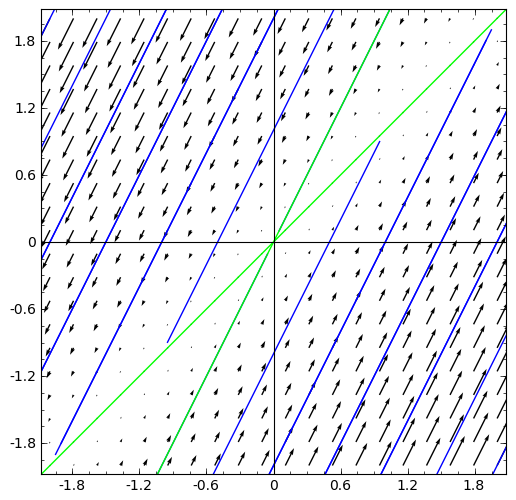
\includegraphics[width=\myvfwidth]{Applications/support/vfi}
\item $-1+i, (1,-i),  -1-i, (1,i)$\\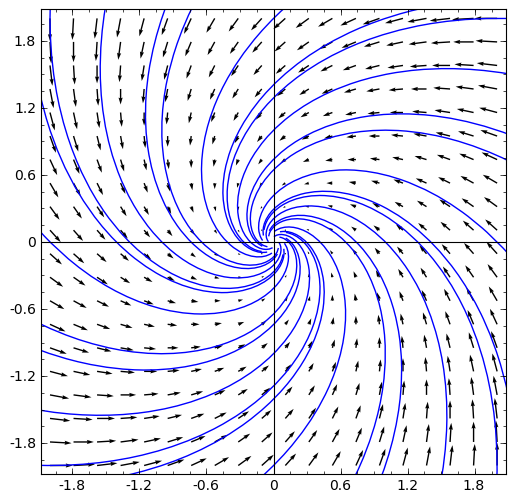
\includegraphics[width=\myvfwidth]{Applications/support/vfj}
\end{enumerate}


\item Kirchoff's Laws

 $\begin{bmatrix}[lll|l]
 1 & -1 & -1 & 0 \\
 R_1 & R_2 & 0 & E \\
 0 & -R_2 & R_3 & 0
\end{bmatrix}$

\begin{enumerate}
\item $(4,2,2)$
\item $(24/7,12/7,12/7)$
\item $(3,2,1)$
\item $(6,3,3)$
\item $(27/11,18/11,9/11)$
\item $(18/5,12/5,6/5)$

$\begin{bmatrix}[llllll|l]
 1 & -1 & -1 & 0 & 0 & 0 & 0 \\
 0 & 0 & 1 & -1 & -1 & 0 & 0 \\
 0 & 0 & 0 & 1 & 1 & -1 & 0 \\
 R_1 & R_2 & 0 & 0 & 0 & 0 & E \\
 0 & -R_2 & R_3 & R_4 & 0 & R_6 & 0 \\
 0 & 0 & 0 & -R_4 & R_5 & 0 & 0
\end{bmatrix}$

\item $\left\{7, 5, 2, 1, 1, 2\right\}$

\item $\left\{\frac{25}{6},\frac{11}{3},\frac{1}{2},\frac{1}{6},\frac{1}{3},\frac{1}{2}\right\}$
\end{enumerate}


\item Cramer's rule
\begin{enumerate}
\item $\left\{\frac{3}{7},-\frac{2}{7}\right\}$
\item $\left\{\frac{5}{2},-\frac{1}{2}\right\}$
\item $\{2,0\}$
\item Fails. The determinant of the coefficient matrix is zero.
\item $\left\{\frac{1}{2},-\frac{1}{2},-\frac{1}{2}\right\}$
\item $\left\{\frac{5}{2},\frac{1}{4},-\frac{9}{4}\right\}$
\item Fails. The determinant of the coefficient matrix is zero.
\end{enumerate}





\item Interpolating Polynomials
\begin{enumerate}
\item $1/2 x + 3/2$
\item $(4/3)x^2-(5/3)x+1$
\item $x^2-2x+2$
\item $(1/4)x^2-(1/2)x+9/4$
\item $(1/8)x^2+15/8$
\item $-x^3+(5/2)x^2+(1/2)x+1$
\end{enumerate}


\item Regression (Make the plots using technology)
\begin{enumerate}
\item $y=\frac{5 x}{2}$
\item $y=\frac{x}{2}+\frac{1}{3}$
\item $y=\frac{7}{4}-\frac{x}{4}$
\item $y=\frac{10 x}{9}+\frac{5}{6}$
\item $y=\frac{5}{2}-\frac{5 x}{3}$
\item $y=\frac{3 x}{7}+\frac{19}{7}$
\item 
$
A=
\begin{bmatrix} 
 0 & 0 & 1 \\
 1 & 1 & 1 \\
 1 & 1 & 1 \\
 16 & 4 & 1
\end{bmatrix},
B=
\begin{bmatrix} 
 0 \\
 3 \\
 2 \\
 5
\end{bmatrix},
A^T A=
\begin{bmatrix} 
 258 & 66 & 18 \\
 66 & 18 & 6 \\
 18 & 6 & 4
\end{bmatrix},
A^T B=
\begin{bmatrix} 
 85 \\
 25 \\
 10
\end{bmatrix}$,

$y=-\frac{5}{12}x^2+\frac{35}{12}x+0
$
\end{enumerate}






%\item Partial Fractions
%\begin{enumerate}
%\item $-1/5\,\ln  \left( x+2 \right) +1/5\,\ln  \left( x-3 \right)$
%\item $1/5\,\ln  \left( x+2 \right) +9/5\,\ln  \left( x-3 \right) $
%\item $1/3\,\ln  \left( x+1 \right) +2/3\,\ln  \left( x-2 \right) $
%\item ${x}^{-1}+3/2\,\ln  \left( x-2 \right) -1/2\,\ln  \left( x \right)$
%\item $-\frac{1}{10}\ln  \left( {x}^{2}+1 \right) -\frac{2}{5}\arctan \left( x \right) +\frac{1}{5}\ln  \left( x-2 \right) $
%\item $-{x}^{-1}-1/2\,\ln  \left( {x}^{2}+1 \right) -\arctan \left( x
% \right) +\ln  \left( x \right)
%$
%\end{enumerate}



\item Second Derivative Test
\begin{enumerate}
\item At $(0,0)$ eigenvalues are $3,1$ (both positive so min) with eigenvectors $[1,1]^T,[-1,1]^T$.
\item At $(0,0)$ eigenvalues are $6,-2$ (saddle point) with eigenvectors $[1,1]^T,[-1,1]^T$.
\item At $(0,0)$ eigenvalues are $4,0$ (test fails) with eigenvectors $[1,1]^T,[-1,1]^T$.
\item At $(2,-1)$ eigenvalues are $2,2$ (both positive so min) with eigenvectors $[1,0]^T,[0,1]^T$.
\item At $(4/3,-2/3)$ eigenvalues are $3,1$ (both positive so min) with eigenvectors $[1,1]^T,[-1,1]^T$.
\item At $(0,0)$ eigenvalues are $6.23607,1.76393$ (both positive so min) with eigenvectors $[.236,1]^T,[-4.236,1]^T$.
\item 
At $(-1,1)$ eigenvalues are $-6,2$ (saddle) with eigenvectors $[1,0]^T,[0,1]^T$.
At $(1,1)$ eigenvalues are $6,2$ (both positive so min) with eigenvectors $[1,0]^T,[0,1]^T$.
\item 
At $(-1,0)$ eigenvalues are $-6,-6$ (both negative so max) with eigenvectors $[1,0]^T,[0,1]^T$.
At $(-1,2)$ eigenvalues are $-6,6$ (saddle) with eigenvectors $[1,0]^T,[0,1]^T$.
At $(1,0)$ eigenvalues are $6,-6$ (saddle) with eigenvectors $[1,0]^T,[0,1]^T$.
At $(1,2)$ eigenvalues are $6,6$ (both positive so min) with eigenvectors $[1,0]^T,[0,1]^T$.

\end{enumerate}






\item Markov Processes

\begin{enumerate}
\item Transition matrix 
$\begin{bmatrix}
 0.85 & 0.1 & 0.15 \\
 0.1 & 0.7 & 0.25 \\
 0.05 & 0.2 & 0.6
\end{bmatrix}$,
5 years  (41.5,32.5,26), 
10 years: (42.425,33.4,24.175),
Steady state: $[4,3,2]^T$ so 4/9 or 44.4\% will be residential. 

\item
Transition matrix 
$\begin{bmatrix}
 {3}/{5} & {1}/{5} \\
 {2}/{5} & {4}/{5}
\end{bmatrix}$,
1 week  (64,136), 
2 week: (65.6,134.4),
3 week: (66.24,133.76),
Steady state: $[1,2]^T$ so 1/3 (33.3\%) will be in Rexburg. This means 66 or 67 cars will be in Rexburg. 
 
\item 
Transition matrix 
$\begin{bmatrix}
 {2}/{5} & {1}/{5} \\
 {3}/{5} & {4}/{5}
\end{bmatrix}$,
1 week  (52,148), 
2 week: (50.4,149.6),
3 week: (50.08,149.92),
Steady state: $[1,3]^T$ so 1/4 or 25\% will be in Rexburg. This means 50 cars will be in Rexburg. 

\item 
Transition matrix 
$\begin{bmatrix}
 {7}/{10} & {1}/{5} \\
 {3}/{10} & {4}/{5}
\end{bmatrix}$,
1 week  (70,130), 
2 week: (75,125),
3 week: (77.5,122.5),
Steady state: $[2,3]^T$ so 2/5 or 40\% will be in Rexburg. This means 80 cars will be in Rexburg. 

\item My order is hamburger, pizza/salad, special (your order may vary which means your matrix will be a little different, but the eigenvector will still have the same ratios).
Transition matrix 
$\begin{bmatrix}
 {3}/{10} & {2}/{5} & {3}/{10} \\
 {2}/{5} & {3}/{10} & {1}/{5} \\
 {3}/{10} & {3}/{10} & {1}/{2}
\end{bmatrix}$,
Steady state: $[29,26,33]^T$ or $[29/88,26/88,33/88]^T$ so Hamburger - 32.9545\%, Pizza/Salad - 29.5455\%, Special - 37.5\%. 

\end{enumerate}







\item  {\bf Column and Row Spaces:} 

\begin{enumerate}
\item Col: 
$\{  (2, -3), (3, -5)  \}$,
$\{  (1, 0), (0, 1),  \}$.
\\Row:
$\{  (1, 0, 14), (0, 1, -9)  \}$,
$\{  (2, 3, 1), (-3, -5, 3)  \}$.

\item Col: 
$ \{  (2, 1),  (1, 3)  \} $,
$ \{  (1, 0), (0, 1)  \} $.
\\Row:
$ \{  (1, 2, 0), (0, 0, 1)  \} $,
$ \{  (2, 4, 1), (1, 2, 3)  \} $.

\item Col: 
$ \{  (1, 2, -3), (2, 0, -2)  \} $,
$ \{  (1, 0, -1), (0, 1, -1)  \} $.
\\Row:
$ \{  (1, 0, 1/2), (0, 1, 5/4) \} $,
$ \{  (1, 2, 3), (2, 0, 1)  \} $.

\item Col: 
$ \{  (1, 2, -3), (3, 1, -4)  \} $,
$ \{  (1, 0, -1), (0, 1, -1)  \} $.
\\Row:
$ \{  (1, 0, -(2/5)), (0, 1, 4/5)  \} $,
$ \{  (1, 3, 2), (2, 1, 0) \} $.

\item Col: 
$ \{  (2, 1, -2), (1, 3, 1), (-2, 0, 1) \} $,
$ \{  (1, 0, 0), (0, 1, 0), (0, 0, 1)  \} $.
\\Row:
$ \{  (1, 0, 0, -1), (0, 1, 0, 2), (0, 0, 1, -2)  \} $,
$ \{  (2, 1, -2, 4), (1, 3, 0, 5), (-2, 1, 1, 2)  \} $.

\item Col: 
$ \{  (0, 2, -1), (1, -1, 2), (3, 0, 5)  \} $,
$ \{  (1, 0, 0), (0, 1, 0), (0, 0, 1)  \} $.
\\Row:
$ \{  (1, 0, -1, 0), (0, 1, 2, 0), (0, 0, 0, 1)  \} $,
$ \{  (0, 1, 2, 3), (2, -1, -4, 0) \} $.

\end{enumerate}


\item  {\bf Coordinates of a vector relative to a basis:} The basis vectors are the pivot columns of rref. See 8 for the basis vectors. To get the coordinates, augment $A$ by the two vectors, and row reduce. 
\begin{enumerate}
\item  
$\vec v: (13, -8)$,
$\vec w: (4, -3) $

\item  
$\vec v: (3, 0)  $,
$\vec w: (-(6/5), 7/5)$

\item  
$\vec v: (-2, 5/2) $,
$\vec w: $ not in space.

\item  
$\vec v: (-3, 2)$,
$\vec w: (-(12/5), 9/5)$

\item  
$\vec v: (-4, 4, -2)$,
$\vec w: (0, -3, 5)$

\item  
$\vec v: (1, 2, -3) $,
$\vec w: (3, -5, -1) $

\end{enumerate}



\item  {\bf Null Space, Eigenspace, and Orthogonal Complement:} There is more than one way to pick a basis. Here possible answers. I obtained these basis by writing solutions in terms of the free variable (rrefing $A$ or $A^T$) and then multiplying by the least common denominator to eliminate fractions.
\begin{enumerate}
\item $\{ (1, -3, 3)\}$
\item $\{ (1, 0, -3, 2), (-2, 1, 0, 0)\}$
\item $\{ (-2, -1, 0, 2), (-4, 1, 2, 0)\}$
\item $\{ (1, -1, 1)\}$

\item $\{ (1, 2, 6)\}$
\item $\{ (12, -8, 0, 7), (2, 1, 7, 0)\}$
\item $\{ (-7, -2, 6)\}$
\item $\{ (1, 2, 0, 3), (-7, -2, 6, 0)\}$

\item $\{ (1, 0, 1), (-1, 1, 0)\}$
\item $\{ (1, 0, 1), (4, 3, 0)\}$

\end{enumerate}



\item {\bf Projections:} The work is identical to problem \ref{regression}. The only difference is the vocabulary. I'll give the coordinates of $\vec w$ as well as $\vec w$
\begin{enumerate}
\item 
Coor: $(0,5/2)$,\\
$\vec w = 5/2(0,1,1)$

\item 
Coor: $(1/3, 1/2)$,\\
$\vec w = 1/3(1,1,1)+1/2(1,2,3)$

\item 
Coor: $(7/4, -1/4)$,\\
$\vec w = 7/4(1,1,1)-1/4(1,3,5)$

\item 
Coor: $(5/6,10/9)$,\\
$\vec w = 5/6(1,1,1,1)+10/9(0,1,1,4)$

\item 
Coor: $(5/2,-5/3)$,\\
$\vec w = 5/2(1,1,1,1)-5/3(0,1,1,4)$

\item 
Coor: $(19/7, 3/7)$,\\
$\vec w =19/7(1,1,1,1)+3/7(-1,1,2,3)$

\end{enumerate}










	
\end{enumerate}


\end{multicols}
}




